\documentclass[12pt]{article}
\usepackage[paper=a4paper,margin=1in]{geometry}
\usepackage[utf8]{inputenc}
\usepackage{amsmath}
\usepackage{amssymb}
\usepackage{enumerate}
\usepackage[ruled,vlined]{algorithm2e}
\usepackage{mathtools}
\usepackage{listings}
\usepackage{tikz}
\usepackage{graphicx}
\usepackage{float}
\graphicspath{{plot/}}

\author{Ibarra Moreno Gisselle }
\title{Colonia de Hormigas\\Heurísticas}

\begin{document}
	\maketitle
	
	\section{Introducción}
	\subsection{Capacitated Vehicle Routing Problem (CVRP)}
	
	El problema de CVRP, es un problema de optimización combinatoria que plantea la
	siguiente pregunta:
	
	Dado un depósito que ofrece un servicio de paquetería, un conjunto de clientes a
	los cuáles se les debe realizar entregas de paquetes, de un tamaño o capacidad $c_i$, un grupo de vehículos con una capacidad $C$ para realizar las entregas, 
	¿Cuáles son las rutas óptimas que deben seguir los vehículos para entregar todos
	los paquetes?
	
	Se puede representar como una gráfica completa $G=(V,E)$ donde $V$ el conjunto 
	de vértices, representa los clientes y el depósito, $E$ las aristas son las
	distancias entre cada par de clientes y las distancias entre el depósito y los
	clientes.
	
	Este problema es una generalización del problema de TSP, en el que se quieren
	encontrar ciclos ajenos con un costo óptimo, con la condición de que el punto de
	partida de todos los ciclos es el mismo. Además la suma de las capacidades que
	requieren los vértices en un ciclo, no deben superar la capacidad $C$.
	
	La función objetivo a optimizar se muestra a continuación:
	\[f(S)=\sum_{t_i \in S}f_t(t_i)\]
	\[f_t(t)=\sum_{i=1}^{n-1}\sum_{j=i+1}^{n}d(i,j)\cdot x_t(i,j) \]
	
	Donde $d(i,j)$ representa la distancia euclidiana entre los vértices $i,j$ y 
	$x_t(i,j)$ representa:
	
	\[x_(i,j)=
	\begin{cases}
		1&\quad\text{si el vehículo $t$ tiene la arista $(i,j)$}\\
		0 & \quad\text{en otro caso}
	\end{cases}\]
	
	Además para que la solución sea factible se debe cumplir que:
	
	\[\forall t\in S \left( \sum_{i=1}^{n}c(i) 
	\right) \leq C\] 
	
	\[c(i)=
	\begin{cases}
		c_i&\quad\text{si el vehículo $t$ tiene el vértice $i$ }\\
		0 & \quad\text{en otro caso}
	\end{cases}\]

	Donde $c_i$ es la capacidad que necesita el paquete a entregar en el vértice $i$.
	
	Se eligió representar las soluciones mediante diccionarios que utilizan como 
	llave el número de vehículo y como valor la ruta que toma el vehículo, sin 
	incluir el depósito.
	Por ejemplo:
	\[\{1:[2,4,12,3], 2:[14,20,2,4,21], 3:[9,5,7,16,10,19], 4:[18,6,8,11,13], 
	5:[17,15]\}\]
	

	\subsection{Colonia de Hormigas (ACO)}
	
	La heurística ACO está basada en el comportamiento real que tienen las hormigas
	para formar caminos entre su hormiguero y las fuentes de comida que encuentran.
	
	La inteligencia enjambre se refiere al comportamiento de organismos que siguen
	reglas simples para interactuar con su medio y otros organismos, estas 
	interacciones derivan en comportamientos más complejos que pueden resolver 
	problemas complicados.
	
	Las hormigas exploran el área cercana a su hormiguero en busca de comida, al
	moverse las hormigas dejan un rastro de feromonas, este rastro lo pueden detectar
	otras hormigas y dependiendo de la concentración de feromonas las hormigas 
	seguirán ese rastro. Cuando la hormiga encuentra una fuente de comida, toma un 
	poco y regresa al hormiguero dejando una concentración de feromonas en el camino
	que depende de la calidad y cantidad de alimento que encontró.
	Esto provoca que varias hormigas sigan su rastro al alimento, dejando más 
	feromonas en el camino y atrayendo más hormigas.
	
	Las hormigas artificiales de la heurística,modelan una solución mediante caminos
	en una gráfica, es muy importante modelar bien la gráfica  que utilizarán las 
	hormigas para construir sus caminos.Las hormigas empiezan siempre a partir del 
	hormiguero, además a diferencia de las reales, sólo dejan feromonas al regresar.
	
	
	El comportamiento que siguen las hormigas artificiales se describe a 
	continuación:

	\begin{enumerate}
		\item En cada iteración cada hormiga construye una solución (camino en la
		gráfica).
		\item Al construir una solución, las hormigas eligen las aristas con una
		probabilidad que depende de la concentración de feromonas en la arista
		\item Al terminar, se actualizan las feromonas de todas las aristas en la 
		gráfica (factor de evaporación).
	\end{enumerate}
	
	Hay muchas variantes de la colonia de hormigas, estas difieren en la forma en que
	se eligen las aristas y la forma en que se actualizan las feromonas de las 
	aristas.
	
	En este proyecto, se utilizó la variante $pseudo-random-proportional$ para la
	construcción de las soluciones, está utiliza un parámetro extra $q_0$. Cada
	hormiga con probabilidad $q_0$ elige la siguiente arista con mayor concentración 
	de feromonas, si no ocurre este evento entonces se eligen con probabilidad 
	uniforme la siguiente arista, esto se ilustra como sigue:
	
	\[e_{i,j}=
	\begin{cases}
		max_{u\in \Gamma(k)}\tau(k,u)&\quad\text{si $q \leq q0$}\\
		\text{J}&\quad\text{si $q > q0$}
	\end{cases}\]

	Donde J es elegida con la siguiente distribución uniforme:

	\[p(e_{i,j})=\frac{\tau_{i,j}}{\sum_{\{k\in \{1,...,|V|\}|v_k\notin T\}}\tau_{i,j}}\]
		
	El factor de evaporación de las feromonas es un número $\rho$,que disminuye un porcentaje de las feromonas de todas las aristas. Esto evita la convergencia 
	prematura en mínimos locales y que la búsqueda no se concentre tan rápidamente 
	en zonas de la gráfica.
	La actualización de feromonas es la siguiente:
	
	\[\tau_{i,j}=\rho \cdot \tau_{i,j} + \sum_{s\in S_{upd}} w_s \cdot F(s)	\]
	
	Donde $S_{upd}$ son las soluciones construidas que tienen la arista $(i,j)$.
	La primera parte de la fórmula ($\rho \cdot \tau_{i,j} $) representa la 
	evaporación de la feromona sobre la arista y la segunda parte ($\rho \cdot 
	\tau_{i,j} $) aumenta el rastro de feromona sobre la arista por cada hormiga 
	que la haya tomado para la construcción de su solución. Además $w_s$ y $F(s)$ son
	factores que determinan la factibilidad y calidad de la solución, siendo $w_s$
	una penalización a la cantidad de feromonas que se agregan si la solución no 
	es factible y $F(s)$ es la función de calidad que nos indica que tan buena es 
	la solución. La adaptación de estos dos elementos para resolver el problema de 
	CVRP se muestra a continuación:
	
	\[w_s=1-(\frac{excess_{St}}{numT})\]
	
	\[F(s)=\frac{f(s)-f(s_{min})}{f(s_{max})-f(s_{min})} \]
	
	Donde $excess_{St}$ es el número de vehículos con su capacidad sobrepasada en 
	la solución y $numT$ el número de vehículos totales.
	
	El pseudocódigo de la colonia de hormigas se muestra a continuación:
	
	\begin{algorithm}[H]
		\SetAlgoLined
		\KwOut{ $s$ mejor solución encontrada }
		\KwIn{$n$ número de hormigas, $G$ gráfica, $q_0$ probabilidad de elegir la mejor arista.}
		$C=inicializaColonia(n)$\\
		\While{not condición de término}{
			$C.construyeSoluciones(G)$\\
			$G=C.actualizaFeromonas(q0)$
			\
		}
		$s=C.mejorSolucion()$\\
		\Return{$s$}
		\caption{Ant Colony Optimization}
	\end{algorithm}
	\section{Implementación}
	La heurística se implementó en el lenguaje Nim.
	Los vehículos representados por la clase $Truck$ tienen un atributo $route$ la cuál es una lista con los ids de los clientes a los que tendrá que llevar una entrega,
	un atributo $cst$ que representa la distancia total que recorre el vehículo para
	repartir todas las entregas y un atributo $capacity$ que representa cuanto 
	espacio tiene para guardar las demandas de los clientes.
	Al crearse la colonia, se inicializan la hormigas, estás se encuentras en un 
	atributo $ants$ que es una lista.
	Las hormigas representan una solución de la heurística, tienen una atributo 
	$trucks$ que es un diccionario en el que se guardan los vehículos del problema.
	Cuando se inicializa una hormiga, esta se crea como una solución aleatoria, es 
	decir, para cada demanda de los clientes, se elige un vehículo de manera 
	aleatoria y se guarda al final de su ruta, de esta manera se construyen rutas
	para cada vehículo y se obtiene una solución para la hormiga.
	
	Con estas hormigas, se hace la primera actualización de las feromonas de la 
	gráfica. A partir de la siguiente iteración se construyen de forma distinta las
	soluciones, ya que se tiene la información obtenida por las soluciones de la 
	primera iteración. Las hormigas utilizan la fórmula vista en la sección anterior 
	para construir su solución; se selecciona un vehículo de forma aleatoria, donde 
	los vehículos con menor número de clientes en su ruta tienen una mayor 
	probabilidad de ser elegidos, mientras que los vehículos con más clientes tienen 
	una probabilidad reducida, de esta manera nos podemos asegurar que no habrán 
	vehículos vacíos. Luego se genera un número aleatorio $q$ el cuál si es menor
	al parámetro $q_0$, entonces se elige la demanda del cliente que tenga la arista
	con mayor nivel de feromonas. En caso de que no se cumpla esto, se calculan las
	probabilidades basadas en el nivel de feromonas, de elegir alguna de las 
	demandas. Las aristas con mayor nivel de feromonas tendrán mayor probabilidad de
	ser elegidas que las aristas con pocas feromonas.
	Al elegirse la demanda, se agrega el costo de tomar esa demanda como parte de la
	ruta del vehículo al costo de la hormiga; de esta manera, no se tiene que recorrer
	vehículo por vehículo para calcular el costo total.
	
	Para actualizar las feromonas de la gráfica, nuevamente se recorren una a una 
	las hormigas de la colonia y dependiendo de su calidad y cuantos vehículos tienen
	su carga sobrepasada, será la cantidad de feromonas que dejarán en las aristas 
	que incluyen en su solución.
	\section{Resultados}
	
	Se realizaron pruebas de la heurística con instancias del conjunto de 
	pruebas A de Augerat. Las instancias utilizadas son:
	
	\begin{itemize}
		\item \textit{A-n32-k5} (32 clientes y 5 vehículos)
		\item \textit{A-n44-k6} (44 clientes y 6 vehículos)
		\item \textit{A-n60-k9} (60 clientes y 9 vehículos)
	\end{itemize}

	La heurística se ajusta mediante los siguientes parámetros:
	
	\begin{itemize}
		\item El número de hormigas $m$.
		\item El parámetro de exploración $q_0$
		\item El factor de evaporación $rho$
	\end{itemize}
	
	Por lo que se experimentó para valores fijos de hormigas, el comportamiento con
	diferentes valores de $q_0$ y $rho$.
	Para todas las instancias, las mejores soluciones resultantes fueron las que 
	tenían como parámetros $q_0=0.6$ y $\rho=0.75$. La construcción de las soluciones
	con estos parámetros tienden a escoger la arista con más feromona desde el vértice en que se encuentre ya que por $q_0$ la probabilidad está más inclinada a
	escoger las mejores, pero sigue existiendo suficiente exploración a otras 
	regiones del espacio de búsqueda. Además por $\rho$ las feromonas de las aristas
	no decrementarán muy rápidamente evitando la convergencia, las aristas de las 
	soluciones que no sean muy
	buenas o que no sean factibles tendrán muy poco impacto, lo que ayudará a que 
	se modelen soluciones con buenos valores y factibles.
	
	Con estos parámetros se ejecutó la heurística con 100 semillas para las 
	instancias \textit{A-n32-k5} y \textit{A-n44-k6} y 30 semillas para la instancia
	 \textit{A-n60-k9}. Los mejores resultados obtenidos se muestran en la siguiente
	 tabla:
	 
	 \begin{table}[!h]
	 	\centering
	 	
	 	\begin{tabular}{|p{0.12\textwidth}|p{0.10\textwidth}|p{0.13\textwidth}|p{0.07\textwidth}|p{0.07\textwidth}|p{0.12\textwidth}|p{0.12\textwidth}|p{0.11\textwidth}|}
	 		\hline 
	 		Instancia & Semilla & Número de Hormigas & $\displaystyle q_{0}$ & $\displaystyle \rho $ & Iteraciones & Mejor solución & Óptimo \\
	 		\hline 
	 		{\small A-n32-k5} & {\small 5} & {\small 20} & {\small 0.6} & {\small 0.75} & {\small 3000} & {\small 928.6397} & {\small 784} \\
	 		\hline 
	 		{\small A-n44-k6} & {\small 82} & {\small 30} & {\small 0.6} & {\small 0.75} & {\small 7000} & {\small 1154.9925} & {\small 937} \\
	 		\hline 
	 		{\small A-n60-k9} & 24 & {\small 35} & {\small 0.6} & {\small 0.75} & {\small 7000} & 2004.4957 & 1354 \\
	 		\hline
	 	\end{tabular}
	 	
 	\end{table}
	 
	
	A continuación se muestran las gráficas de evolución para cada instancia, se 
	puede notar las mejoras que se fueron dado a lo largo de la ejecución de la 
	heurística para todas las instancias:
	
	\begin{figure}[H]
		\centering
		\caption{Gráfica de evolución de A-n32-k5}
		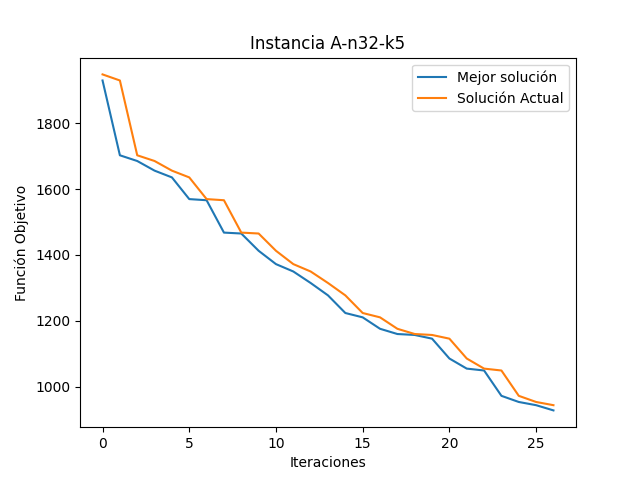
\includegraphics[scale=0.5,width=12cm]{n32-k5.png}
	\end{figure}

	\begin{figure}[H]
		\centering
		\caption{Gráfica de evolución de A-n44-k6}
		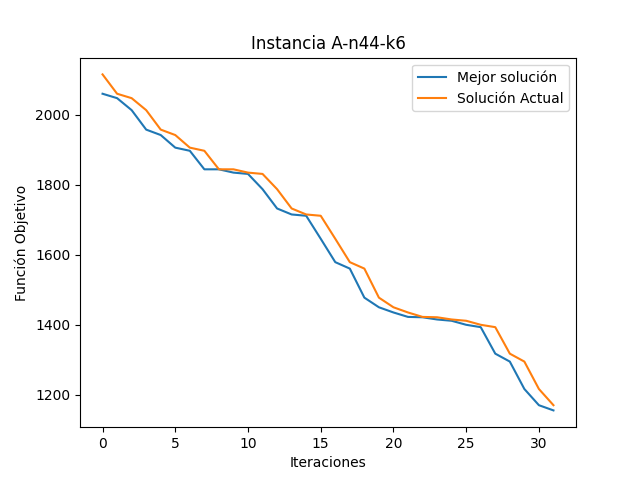
\includegraphics[scale=0.5,width=12cm]{n44-k6.png}
	\end{figure}
	\begin{figure}[H]
		\centering
		\caption{Gráfica de evolución de A-n60-k9}
		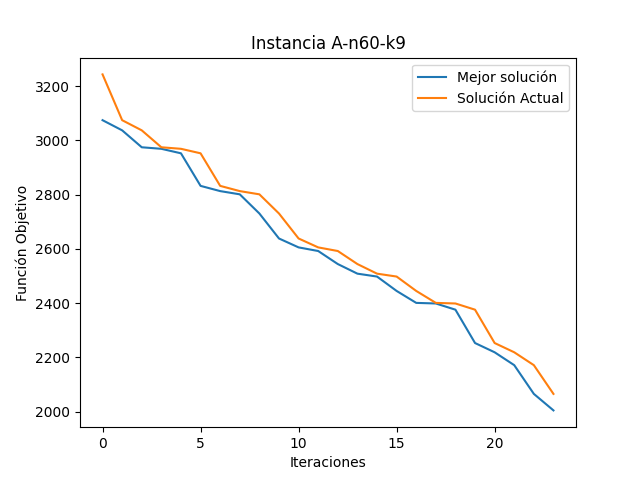
\includegraphics[scale=0.5,width=12cm]{n60-k9.png}
	\end{figure}
	
	\section{Conclusión}

	La heurística tomaba un periodo de tiempo no tan grande para la instancia más 
	pequeña, considerando la cantidad de iteraciones que se ejecuta, para las instancias más grandes, el tiempo que toma la ejecución de una sola semilla es
	alrededor de 5 min.
	Los resultados obtenidos, aunque no fueran el óptimo, son cercanos y factibles. 
	Es posible que con un mayor ajuste a los parámetros $q_0$, $\rho$ y número de 
	hormigas de la heurística, al igual que probar con diferentes valores iniciales
	para las feromonas en la gráfica  y una mayor cantidad de iteraciones, la heurística logre encontrar los óptimos de las instancias.
	\section{Referencias}
	\begin{enumerate}
		\item Silvia Mazzeo, Irene Loiseau, An Ant Colony Algorithm for the Capacitated Vehicle Routing. http://www.sciencedirect.com/science/article/pii/S1571065304010868
		
		\item Christian Blum, Ant colony optimization: Introduction and recent trends.\\
		http://www.sciencedirect.com/science/article/pii/S1571064505000333
		
	\end{enumerate}
\end{document}